
We propose a \textit{design pattern} for building query processing systems,
with the goal of evolving query processing system's architecture from monolithic and static to modular and flexible.
Traditional static query processing systems are not able to cater to the needs of modern applications in which users and
data are geo-distributed across the globe.
Our vision is to enable query processing systems that are designed and deployed on a case-by-case basis,
with the workload characteristics, data and access distribution patterns, and requirements of specific applications in
mind.
As a first step towards this vision, we focus on the \textit{mechanisms} required for enabling a flexible and configurable
query processing system architecture.

\medskip

The key idea for the proposed design pattern \textit{assembly-based modularity}.
The query processing system's architecture is modular:
it is constructed by interconnecting composable building blocks
that encapsulate components of a traditional query processing system such as indexes, materialized views,
and caches, as well as relational operators such as filters, aggregations, and joins.
Modularity translates design decisions about the use of derived state to which building blocks are used and how they are
interconnected.
For example, adding a caching layer to an existing system can be done by extending an existing query system architecture
with additional building blocks.

Moreover, modularity enables configurable placement.
The components of a modular architecture, as opposed to a monolithic one,
can be decoupled from the storage tier, and flexibly placed across the system infrastructure.


\section{Overview: a modular query processing architecture}

According to the design pattern that we propose,
a query processing system is a composition of building blocks that encapsulate query processing tasks, called
Query Processing Units (QPUs).

A QPU is a \textit{system component} that combines properties of a microservice and a streaming operator.
Similarly to a streaming operator, a query processing unit receives one or more input streams,
performs a computation over these streams, and emits an output stream.
Similarly to microservice, a QPU initiates an output stream as a result of receiving a query request;
it can itself send query request to other QPU in order to initiate input streams.

\medskip
\noindent
A query processing unit can implement a \textit{relational operator}.
For example, a ``join operator'' QPU receives input streams that represent the tables to be joined,
and emits an output stream that represents the results of the join operation.

Moreover, a QPU can implement a \textit{derived state structure}, such as an index, a materialized view, or a cache.
For example, a ``secondary index'' QPU receives an input stream that represents notifications for updates to the table
to be attribute to be indexed; it maintains a secondary index data structure, which it stores as internal state.
When it receives a query request, it reads from its internal state and emits the result as an output stream.

Finally, multiple ``secondary index'' QPUs can be used to implement partitions of \textit{partitioned index}
Another type of QPU can be then used to as a ``partition manager''; given a query, the ``partition manager'' QPU sends query
requests to the appropriate  ``index partition'' QPUs, thus initiating input streams; it then combines these input streams
and emits the result as an output stream.

Our key insight all three of the described QPU types --- relational operators, derived state, and routing operators ---
can be generalized to a system component with common semantics, and thus can be composed arbitrarily to implement complex
query processing computations.

\medskip
\noindent
QPUs are organized in a directed acyclic graph:
a QPU can send query requests to other QPUs it has outgoing connections to in the graph (downstream neighbors)
Base data are the leaves of the graph (nodes with only incoming edges),
and client queries enter the graph through its root nodes (nodes with outgoing edges).

When a QPU receives a query, it can process it by reading from its internal state, it can initiate input streams
by sending query requests to its some of its downstream neighbors and produce query results using these streams,
or a combination of the two.
This process is recursively performed at each downstream QPU, creating a query execution tree.

\section{Query Processing Unit: the building block}

\subsection{The Query Processing Unit abstraction}

The key property required by query processing unit to effectively serve as building blocks of the modular query
processing systems is composability:
QPUs should be able to be interconnected in various topologies, and interoperate in the execution of query processing tasks.

To achieve this, we define a common set of properties that any query processing unit should conform to.
This properties include a common interface for receiving query request, and common the interaction semantics among QPUs.
We call this set of properties the query processing unit \textit{abstraction}.
Using object-oriented programming terminology, the QPU abstraction can be viewed as an \textit{abstract class}
that defines a set of methods, but does not include their implementation.
Implementations of the QPU abstraction define \textit{QPU classes} with specific functionalities,
such as join or index QPU classes.
Using the object-oriented programming analogy, QPU classes can be viewed as classes that implement the QPU
abstract class.
Finally, specific \textit{QPU instances} can be viewed as objects of a specific QPU class, for example a index QPU that
indexes the attribute $predominantColor$ of a table $photoAlbum$.
The building blocks of a modular query processing system are QPU instances.

In the rest of this thesis we use the terms query processing unit, QPU, and unit interchangeably to refer to QPU instances.

\bigskip

More specifically, the query processing unit abstraction defines a \textit{system component} with the following properties:

\begin{figure}[t]
  \centering
    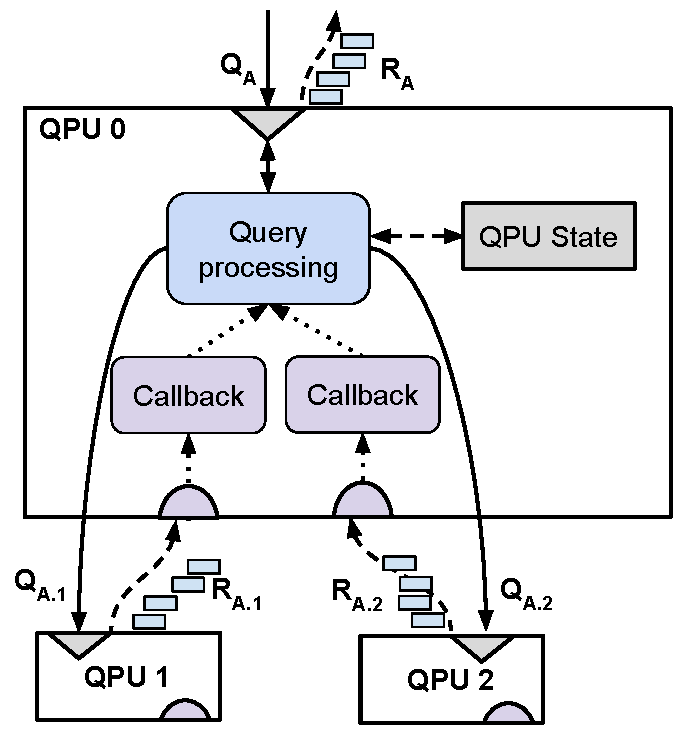
\includegraphics[width=0.5\textwidth]{./figures/design_pattern/qpu_abstraction.pdf}
  \caption{A conceptual depiction the QPU abstraction.}
  \label{fig:qpu_abstraction}
\end{figure}

\medskip
\noindent
\textbf{Query interface.}
Every QPU exposes an interface for receiving query requests.
While this interface is common among all QPUs, QPU classes and specific QPU instances restrict the set of queries
that they can serve.
For example, a QPU may only serve queries about a specific database table.
As a result, QPUs can be though of as microservices that serve queries

The QPU's query interface has \textit{streaming semantics}.
An invocation of the interface establishes between the QPU and caller:
the QPU sends query result entries as stream records; the caller can send control messages such as acknowledgements.
We present the query interface in more detail in section \todo{ref}.

The query interface can be invoked by other query processing units.
This is how QPUs interoperate and forms the basis of the query processing system's computation model \todo{ref}.
We call the act of a $QPU_a$ invoking the query interface of a $QPU_b$, a \textit{downstream query}.

\medskip
\noindent
\textbf{Query processing function.}
Every QPU implements a function that is called when its query interface is invoked, and is responsible for processing
the given query and writing to the query result stream.

The implementation of this computation is specific to each QPU class.

Two capabilities are available for the implementation of the query processing function:
accessing the QPU's state, and initiating input streams by sending query requests to downstream neighbors.

\medskip
\noindent
\textbf{State.}
Each QPU maintains \textit{internal} state, that is accessible only by that specific QPU.

We distinguish the QPU state in three parts according to its functionality.
In this section, we present an overview of the functionality of each state type.
In section~\ref{ref:specification} we present the QPU's state in detail.

Each query processing unit maintains \textit{configuration state} that represents the query processing unit's
configuration parameters.

In addition, each QPU with outwards connections in the QPU graph maintains information about the
\textit{query processing capabilities} of these QPUs. \todo{ref}.
This information is used by the for creating and generating and sending downstream query requests in order to initiate
input streams that it can use during query processing \todo{ref}.

Finally, query processing units that implement derived state structures, and units need to store intermediate query processing
results, for example \todo{in streaming join computation?}, maintain \textit{query processing state}.

\medskip
\noindent
\textbf{Input stream callback function.}
Each QPU implements a callback function that is called for each record received through an input stream.
Similarly to the query processing function, the implementation to callback function is part of the definition of each
QPU class.

\bigskip

A conceptual depiction of the query processing unit abstraction is shown in Figure~\ref{fig:qpu_abstraction}.
When the QPU's query API is called, a response stream ($R_A$) is established between the unit and the client, and
the unit's query processing computation is invoked.
The query processing computation can read the QPU's state, and can perform downstream queries to other units.
For each downstream query, a corresponding stream is established ($Q_{A.1}$ and $Q_{A.2}$).
When a record is received from one of the streams, the QPU's callback computation is invoked.
Each callback computation processes the received record, and returns the result to the query processing computation.
Upon receiving a result from the callback, the query processing computation can write to the QPU's
state and potentially send a computed query result through the response stream.


\subsection{Query Processing Unit specification}
\label{ref:specification}

In this section we present the detailed specific of the Query Processing Unit abstraction.

\subsubsection{Query interface}

In this section, we first present a high level overview of the QPU abstraction's interface,
and then describe each of its elements in more detail.

Each query processing unit exposes and interface for receiving query requests:


\begin{displaymath}
  Query(QueryRequest) \rightarrow QueryResponse
\end{displaymath}

$QueryRequest$ specifies a predicate on the data items' \textit{attributes}, and a \textit{time interval}.

$QueryResponse$ is a stream containing records that represent \textbf{updates} (an update can be a creation, modification, or deletion)
performed to data item of the corpus
It represents updates as \textit{deltas}:
a delta representing an update $u$ contains the data item's attribute values before $u$ is applied,
and those after the $u$ is applied.

More specifically:
\[
  QueryResponse = [UpdateDelta]
\]
where
\[
  UpdateDelta =
\]
\[
  (DataItemID, [(AttributeName, AttributeValue_{old}, AttributeValue_{new})], timestampValue)
\]
\todo{ensure consistent terminology}

An $update$ is a triplet containing
(1) the primary key of the data item ($DataItemID$) it refers to,
(2) a list of triplets of the form $(AttributeName, AttributeValue_{old}, AttributeValue_{new})$ that represent the
data item's attribute values before and after the update is applied,
and (3) the timestamp ($timestampValue$) assigned to the update.

Given a $QueryRequest$ that specifies an attribute predicate $Pred$ and a time interval $T$ $=$ $[t_1, t_2)$
\begin{itemize}

  \item If $t_1$ $=$ $t_2$ = $t$,
  then for each data item $QueryResponseRecord$ contains \textit{only the latest update before $t$},
  provided that after applying that update the data item's attributes satisfy $Pred$.
  We term this case a \textit{snapshot query}.

  \item if $t_1$ $<$ $t_2$,
  then for each data item $QueryResponseRecord$ contains any update with $t_1$ $\leq$ $timestampValue$ $<$ $t_2$,
  provided that the data item's attributes satisfy $Pred$ \textit{either before or after applied that update}.
  We term this case a \textit{an interval query}.

\end{itemize}

A snapshot query, therefore queries a \textit{snapshot} of the corpus that contains the effect of every update with a
timestamp $<$ $t$.
By returning the latest update before $t$, a snapshot query effectively returns that \textit{state} of the data items
that satisfy $Pred$ in the snapshot defined by $t$.

In contrast, an interval query receives for each data item any update within the specified time interval that modifies
the data item so that either is starts of it stops satisfying $Pred$.
By using a $t_2$ in the future, an interval query can continue receiving updates that satisfy $Pred$.
This provides a mechanism for \textit{subscribing to notification for updates based on a given predicate}.

\bigskip

\textbf{Query Language.}
% https://documentation.basis.com/BASISHelp/WebHelp/usr2/sql_grammar.htm
% http://www.h2database.com/html/grammar.html#expression
% $Query$ receives $QueryRequest$ and returns a stream of $QueryResponseRecord$:

The query processing abstraction implements an SQL-like query language,
that supports point and range queries, logical operators, aggregation functions, and joins.

We argue that these is no inherent limitation in the query processing unit abstraction that prevents it from implementing
more complex functionalities, such as nested queries.
However, we consider additional functionalities to be out of the scope of this work.
We believe this query language can effectively demonstrate that the query processing unit abstraction can be used as building
block for constructing fully-functional query processing systems.

The QPU abstraction's query language has following syntax:

{\obeylines\obeyspaces
\texttt{
QueryRequest          ::=  SELECT SelectExpression
~~~~~~~~~~~~~~~~~~~~~~~~~~~FROM TableExpression
~~~~~~~~~~~~~~~~~~~~~~~~~~~WHERE PredicateExpression
~~~~~~~~~~~~~~~~~~~~~~~~~~~TIMESTAMP TimestampExpression \todo{the timestamp can be just another attribute, but I think we need to have it separate for emphasis}
~~~~~~~~~~~~~~~~~~~~~~~~~~~[ GROUP BY attributeName ]
~~~~~~~~~~~~~~~~~~~~~~~~~~~[ ORDER BY OrderByExpression \{ ASC | DESC \} ]
}}

{\obeylines\obeyspaces
\texttt{
SelectExpression      ::=  ALL
~~~~~~~~~~~~~~~~~~~~~~~~~~~SelectExpressionItem , SelectExpression |
~~~~~~~~~~~~~~~~~~~~~~~~~~~SelectExpressionItem
}}

{\obeylines\obeyspaces
\texttt{
SelectExpressionItem  ::=  SUM(attributeName) | AVG(attributeName) |
~~~~~~~~~~~~~~~~~~~~~~~~~~~MAX(attributeName) | MIN(attributeName) |
~~~~~~~~~~~~~~~~~~~~~~~~~~~attributeName
}}

{\obeylines\obeyspaces
\texttt{
TableExpression       ::=  tableName JoinType tableName USING attributeName |
~~~~~~~~~~~~~~~~~~~~~~~~~~~tableName
}}

{\obeylines\obeyspaces
\texttt{
JoinType              ::=  \{ INNER | \{ LEFT | RIGHT \} OUTER \} JOIN
}}

{\obeylines\obeyspaces
\texttt{
PredicateExpression   ::=  PredicateExpression OR PredicateExpression |
~~~~~~~~~~~~~~~~~~~~~~~~~~~PredicateExpression AND PredicateExpression |
~~~~~~~~~~~~~~~~~~~~~~~~~~~NOT PredicateExpression |
~~~~~~~~~~~~~~~~~~~~~~~~~~~Term Op Term
}}

{\obeylines\obeyspaces
\texttt{
Term                  ::=  attributeName | Value
}}

{\obeylines\obeyspaces
\texttt{
Op                    ::= > | >= | < | <= | = | !=
}}

{\obeylines\obeyspaces
\texttt{
Value                 ::= stringValue | floatValue | intValue |
~~~~~~~~~~~~~~~~~~~~~~~~~~dateTimeValue | timestampValue
}}

{\obeylines\obeyspaces
\texttt{
OrderByExpression     ::= attributeName , OrderByExpression |
~~~~~~~~~~~~~~~~~~~~~~~~~~attributeName
}}

{\obeylines\obeyspaces
\texttt{
TimestampExpression   ::= FROM TimestampTerm [ TO TimestampTerm ]
}}

{\obeylines\obeyspaces
\texttt{
TimestampTerm         ::= SYSTEM START | LATEST | timestampValue
}}

~ \bigskip

In practice, each QPU class can only process a subset of the queries that can be expressed by this query language,
according to its functionality.
For example, a QPU class that implements a join operator can perform a only join over two input streams.
Performing an aggregation or applying a predicate over the result of the join requires this use of other QPU classes.

\todo{references: QPU classes, composition / query execution}

Moreover, individual QPUs of a certain class may support different subsets of the query language according to their
configuration.
For example, two instances of a filter operator QPU class may provide predicate queries for different tables.

% % ---- QPUs are able to send query requests to other units (their child nodes in the QPU graph) by invoking their API.

\subsubsection{QPU State}

A query processing unit maintains the following types of state:

\medskip
\noindent
\textbf{Query processing state}
The QPU's query processing state can be used to implement derived state structures, such as indexes, materialized views and
caches.
In addition it can be use for storing intermediate state used in query processing computations.

We model the query processing state as ordered key/value map, in which keys are string values, and values are lists of
data items, represented as:
\[
  (DataItemID, [(AttributeName, AttributeValue)], timestampValue)
\]

Using pseudocode, we can represent the query processing state as follows:

\begin{lstlisting}[caption={Pseudocode for the QPU's query processing state},captionpos=b,label={lst:qpustate}]
type DataItem {
  dataItemID  string
  attributes  [(AttributeName, AttributeValue)]
  ts          timestamp
}

class QueryProcessingState
  function Get(Key_low, Key_high) [(Key, [DataItem])]
  function Put(Key, [DataItem])
\end{lstlisting}

$Get$ retrieves the query processing state entries with $Key_low$ $<$ $key$ $\leq$ $Key_high$.
$Put$ modifies the value of the query processing state for a given key.
It can be used with a non-existing key to create a new entry, or with an empty value to delete an entry.

\medskip
\noindent
\textbf{Configuration state.}
The configuration state represents the configuration parameters passed to a query processing unit when it is created.

The configuration state consists of two types parameters:
\begin{itemize}
  \item Connection parameters.
  The QPU configuration specifies the endpoints of the unit's outwards connections in the QPU graph (downstream neighbors).

  \item Class-specific parameters.
  Instances of a QPU class can have different properties.
  For example, different instances a QPU class that implements a query cache can have different cache sizes.
  These characteristics are defined by the QPU's class-specific configuration.

\end{itemize}
% % This is the part of the state that defines the QPU's behavior (includes its type
% % and neighborhood).
% % Passed as argument during initialization.
% % This type of state is composed of configuration parameters, such as the endpoint of its downstream neighbors.

\begin{lstlisting}[caption={Pseudocode for the QPU's configuration state},captionpos=b,label={lst:qpuconfigstate}]
class ConfigurationState
  function GetConfigParameter(Key) ConfigParameterValue
\end{lstlisting}

\todo{..}

\medskip
\noindent
\textbf{Downstream neighbors' capabilities .}
% This is the part of the state that describes the QPU's knowledge/view of the
% sub-graphs it is connected to.
% It is initialized using the ``getConfig'' API method.
% Each QPU maintains metadata that represent information about its downstream neighbors, such as their QPU class,
% and their capabilities \todo{ref}.
% These metadata is used during query processing for generating downstream query requests \todo{ref}.
\todo{..}

\subsubsection{Query processing function}

% % \begin{algorithm}
% % \caption{Query processing function signature}
% % \label{func:query_processing}
% % \begin{algorithmic}
% % \Function{ProcessQuery}{QueryRequest, State, DownstreamNeigbors, ResponseStream}
% % \end{algorithmic}
% % \end{algorithm}
% Every QPU implements a function that is responsible for processing queries request received by the QPU.
% The query processing function is the core to the query processing unit's functionality.
% As different QPU classes have implement different functionalities, the query processing function's implementation is
% class-specific.


\begin{lstlisting}[caption={Query processing function signature},captionpos=b,label={lst:query_processing_func}]
function ProcessQuery(QueryRequest, State, DownstreamNeighbors, ResponseStream)
\end{lstlisting}

\noindent
Listing~\ref{lst:query_processing_func} shows the query processing function's signature.
$ProcessQuery$ receives the following arguments:
\begin{itemize}

  \item $QueryRequest$, which represent the received query request.
  \item $State$, which allows $ProcessQuery$ to access QPU's state.
%   Listing~\ref{lst:state_object} blah

%     \begin{lstlisting}[caption={The QPU's $State$ object},captionpos=b,label={lst:state_object}]
%     type State {
%       qpState                 QPState
%       config                  Configuration
%       downstreamCapabilities  map[downstreamQPU]Capabilities
%     }

%     type DataItem {
%       dataItemID  string
%       attributes  [(AttributeName, AttributeValue)]
%       ts          timestamp
%     }

%     function (QPState) Get(Key_low, Key_high) [(Key, [DataItem])]
%     function (QPState) Put(Key, [DataItem])

%     function (Configuration) GetConfigParameter(Key) ConfigParameterValue

%     \end{lstlisting}


  \item aaa
\end{itemize}




% \begin{lstlisting}[caption={TODO},captionpos=b]
% struct DownstreamNeighbors {

% }
% \end{lstlisting}

% \begin{lstlisting}[caption={TODO},captionpos=b]
% struct ResponseStream {

% }
% \end{lstlisting}




% % The query processing function's implementation is specific to each QPU class
% % the given query and writing to the query result stream.

% The implementation of this computation is specific to each QPU class.

% Two capabilities are available for the implementation of the query processing function:
% accessing the QPU's state, and initiating input streams by sending query requests to downstream neighbors.


% \subsubsection{Input stream callback function}

% Each QPU implements a callback function that is called for each record received through an input stream.

% ... The implementation of this computation is may differ between QPU classes ...

% % \begin{algorithm}
% % \caption{Input stream callback function}
% % \label{func:callback}
% % \begin{algorithmic}
% % % \Function{ProcessQuery}{QueryRequest, State, DownstreamNeigbors, ResponseStream}
% % \end{algorithmic}
% % \end{algorithm}

% \subsection{QPU classes (overview)}
% \label{sec:qpu_classes}

% % As described earlier, the QPU abstraction works as a ``blueprint''.
% % It specifies a communication and execution protocol that QPUs must conform to.
% % However, there can be different instantiations of this specification.
% % We term these instantiations of the QPU abstraction, classes.

% % More specifically, each QPU class defines:
% % \begin{itemize}
% %   \item The query processing state of the units is this class.
% %   \item Their query processing and callback functions.
% % \end{itemize}

% % We categorize QPU classes in three distinct families:
% % \begin{itemize}
% %   \item \textbf{Stateful QPUs}. QPU classes of this family maintain internal
% %   query processing state and use it to process queries.
% %   Examples include index, cache, and materialized view QPUs.
% %   \item \textbf{Stateless QPUs}. QPU classes of this family do no maintain
% %   internal query processing state (or maintain only intermediate state).
% %   Stateless (or Functional ?) QPUs process queries by performing computation on
% %   incoming streams (they initiate streams by sending queries to other QPUs.)
% %   Examples include filter, join, and aggregation QPUs.
% %   \item \textbf{Routing QPUs}. Stateful and stateless QPUs can only have a
% %   single outgoing (child) connection in the QPU graph.
% %   TODO: QPU graph has not been defined until point. Define-before-reference.
% %   Routing QPUs have multiple outgoing connections.
% %   They are responsible for re-writing incoming to queries to sub-queries,
% %   sending them to the appropriate child QPUs, and merging the responses to a
% %   single outgoing response stream.
% %   Routing QPUs can be used for example to build sharded indexes by composing
% %   multiple index QPUs.
% % \end{itemize}

% \section{QPU Composition: Constructing QPU-based query engines}
% Here, describe how query engines are constructed using instances of QPU classes.

% A query engine is a directed acyclic graph (why?) with QPUs as nodes.

% Describe the QPU-specific topology properties that the graph must satisfy in
% order to be functional:
% \begin{itemize}
%   \item All leaves must be QPUs of the datastore driver class.
%   Also, datastore driver QPUs cannot be nodes other than leaves.
%   \item TODO
% \end{itemize}

% \section{Computation Model}
% Describe the bidirectional data-flow computation.
% \begin{itemize}
%   \item Control messages (queries) flow downwards.
%   \item Responses flow upwards through the sub-graph defined by the control
%   (each query establishes a sub-graph - actually a tree - to be used by that
%   particular query);
%   \item Updates (independently) also flow upwards.
% \end{itemize}


% % \section{The consistency guarantees of QPU-based query engines}
% % TODO: What mechanism are needed so that QPUs can guarantee internal consistency?
% % What about session consistency guarantees?

% \section{Discussion}

% % -- point to make -- unified subscription and snapshot

% % It is known that query execution can be represented as a tree.
% % Base data are at the tree's leaves, tree nodes are relational operator such
% % as filter, joins and aggregations, and query result are at the root of the tree.
% % Each operator receives an input stream of records, performs a transformation on the, and emits a output stream of record.
% % This results to a data-flow computation in which data items flow upwards through the tree and are progressively transformed
% % to the query execution results.

% % Computation tasks vs architecture components

% % Our approach is based on three simple insights:
% % \begin{itemize}
% %     \item \textbf{Index-based distributed query processing is composed of basic, primitive tasks.}
% %     The most simple query engine design is a component that scans the corpus dataset and selects the data items which match a given query.
% %     When queries for certain attributes are frequent or require low response time, secondary indexes can be materialized for those attributes.
% %     Even when indexes are partitioned and distributed across the system for scalability, the basic components of an indexing system remains the same: index data structures that collaborate through appropriate index maintenance and query processing protocols to implement distributed indexes.
% %     Additional query processing functionalities such as multi-attribute queries, joins or federated queries across multiple corpus can be implemented using operators that build on top of these components.
% %     Finally, caching can be used to further improve response time for certain queries.

% %     \item \textbf{Primitive query processing tasks can be encapsulated by a common query processing component abstraction.}
% %     Each of the described tasks can be encapsulated by a query processing component abstraction with two properties: an API for responding to queries, and a callback function.
% %     For example, index data structures in general implement three basic functions: LOOKUP, INSERT, DELETE.
% %     The query API can encapsulate the LOOKUP function, while the callback function can express the task of index maintenance, receiving corpus updates and updating the index accordingly, and therefore encapsulate INSERT and DELETE.
% %     As another example, a cache on top of an index structure should be able to respond to the same queries as the underlying index, and therefore can be encapsulated by a query processing component with the same query API.
% %     Similarly, its callback function can express the task of receiving query results in case of a cache miss, and updating the cache.
% %     This concept can be generalized to represent other query processing components including bloom filters, materialized views, and streaming operators.

% %     \item \textbf{Query processing components need to cooperate to implement complex query processing tasks.}
% %     As an example, a caching component requires the ability to forward queries to other components, such as indexes, when cache misses occur.
% %     Similarly, a distributed indexing system, in which indexes are partitioned and distributed across system nodes, can be implemented using indexing components with the help of an additional component responsible for implementing a partitioned LOOKUP operation, by collecting and aggregating partial LOOKUP results.
% % \end{itemize}

% % Based on these observations, we introduce a query processing component abstraction, called the \textit{Query Processing Unit} (QPU).
% % We have designed a generic query API and callback function interface with the aim of encapsulating multiple different query processing components.
% % Query processing units may have internal state for facilitating query processing, or be stateless.
% % Additionally, QPUs have the ability to invoke the query API of one another, and thus interoperate for query processing.
